\documentclass[oneside,a4paper,12pt]{article}
\usepackage{graphicx}
\usepackage[section]{placeins}
\usepackage{listings}
\graphicspath{{~/templates/}, {../images/}}

\makeindex
\begin{document}
	\begin{titlepage}
		\includegraphics[width=4cm]{logopopo.png}
		\hspace*{\fill}
		\includegraphics[width=6cm]{univlille.png}
		
		\begin{center}
			\vspace{1cm}
			\textbf{TP Traitement du Signal}\\
			\textbf{Analyseur de spectre haute fréquence}\\
			\vspace{1cm}
			\textbf{Valentin DOSIAS, Maxence NEUS}\\
			\vspace{3cm}
			%\includegraphics[width=13cm]{titlepage.png}\\
			\vspace{\fill}
			\textbf{Decembre 2021}\\
		\end{center}
	\end{titlepage}
	
	\tableofcontents
	
	\vspace{5cm}
	
	\section{Introduction}
	
	L’objectif de ce TP est de calculer avec le logiciel les transformées de Fourier de différents signaux avec les différents paramètres que propose le logiciel et de les comparer avec les résultats théoriques. 
	\newpage
	
	\section{Signal sinusoidal}
	
	\paragraph{Théorie}\paragraph{}
	Nous avons 
	$$ TF(sin(2 \pi f t)) = \frac{1}{2 j}F(e^{2 \pi f_{0} t} - e^{-2 \pi f_{0} t}) $$
	Or par définition du pic de Dirac nous avons
	$$ F(e^{2 \pi f_{0} t})=\delta(f-f_{0}) $$
	Ainsi 
	$$ TF(sin(2 \pi f t)) = \frac{1}{2j}*(\delta(f-f_{0})-\delta(f+f_{0})) $$
	Nous devrions obtenir un pic de Dirac d’amplitude $-\frac{A}{2}$ à $-f_{0}$ et un pic d’amplitude $\frac{A}{2}$ à $f_{0}$. Or nous devons prendre en compte que les appareils de mesures en général et le logiciel de ce tp n’affichent que les fréquences et amplitudes positives.
	
	\paragraph{Pratique}\paragraph{}
	Nous étudions d’abord un signal sinusoïdal composé de 8 échantillons. La fréquence d’échantillonnage est de 800 Hz. 
	
	\begin{figure}[h]
		\centering
		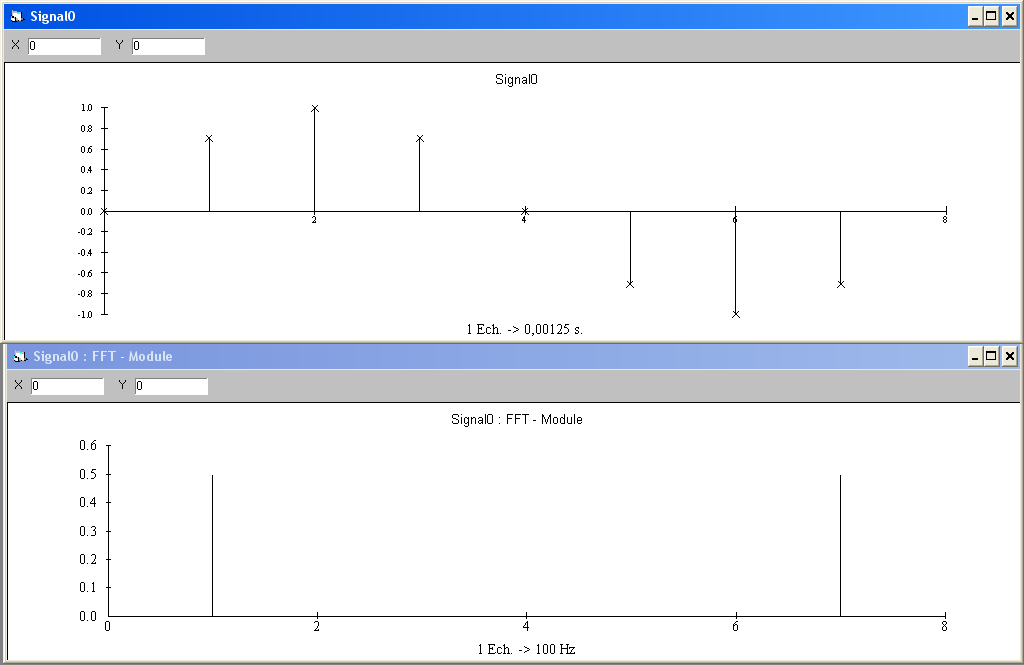
\includegraphics[width=10cm]{fig1.png}
		\caption{Sinus 100Hz, 8 échantillons}
	\end{figure}

	Le résultat est en accord avec la théorie, nous obtenons bien deux pics de Dirac. Le deuxième est bien celui que nous devrions avoir dans la partie négative en théorie. Cependant en réalité les appareils de mesures n’ont pas de partie négative, le pic apparaît donc dans la partie positive à $f_{echantillonage}-f_{signal} = 700 Hz$. Nous retrouvons bien l’amplitude du signal en additionnant l’amplitude des deux pics.
	
	\begin{figure}[h]
		\centering
		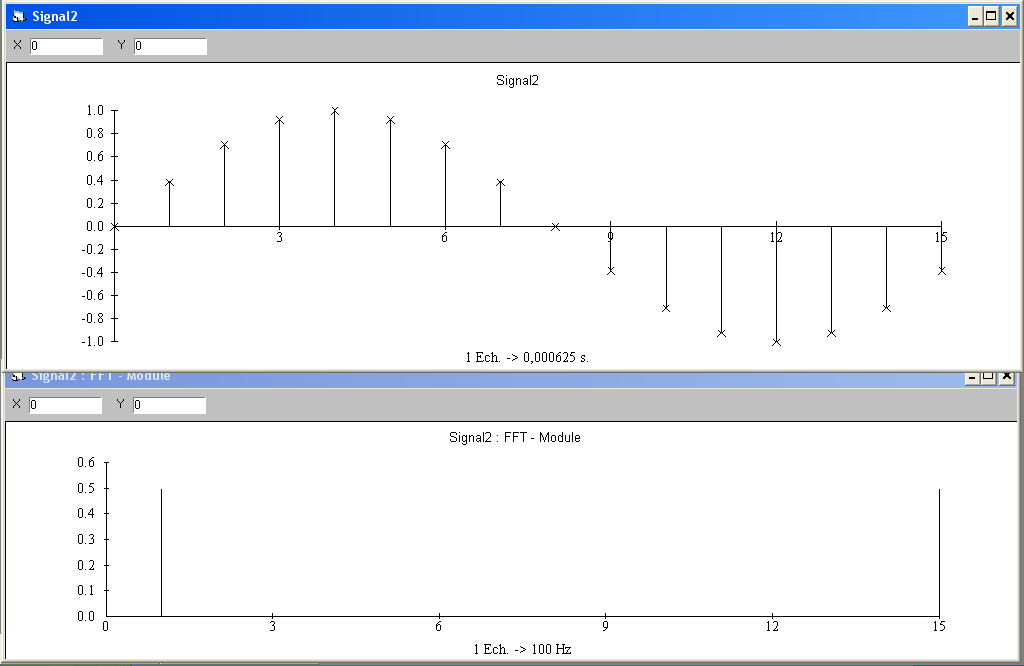
\includegraphics[width=12cm]{fig2.PNG}
		\caption{Sinus 100Hz, 16 échantillons}
	\end{figure}

	Ici nous avons augmenté la fréquence d'échantillonnage et le nombre d'échantillons, le résultat est le même et est toujours en accord avec le résultat théorique.\\
	\newpage
	
	\begin{figure}[t]
		\centering
		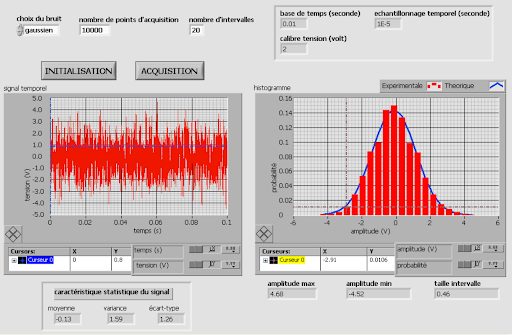
\includegraphics[width=12cm]{fig3.png}
		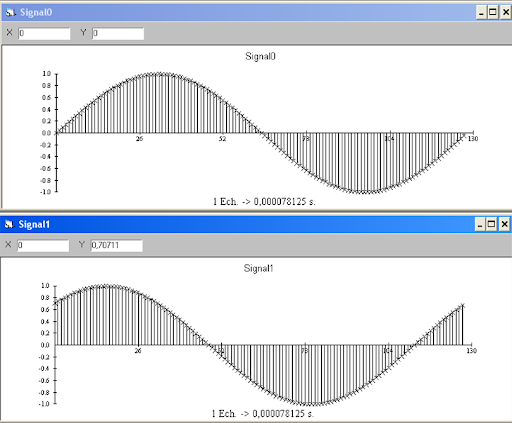
\includegraphics[width=12cm]{fig4.png}
		\caption{Sinus 100Hz, 16 échantillons, 2 périodes}
	\end{figure}

	Nous avons fait la transformée avec deux périodes et une fréquence d’échantillonnage de 800 Hz. Le résultat est toujours en accord avec la théorie. Nous retrouvons les deux pics aux bonnes fréquences et la somme de leur amplitude vaut bien l’amplitude de notre signal. Le changement de la transformée ne pourrait être que provoqué par un changement de la fréquence d’échantillonnage qui décalerait le second pic de Dirac.
	
	\newpage
	
	\section{Signal Continu}
	
	\paragraph{Théorie}\paragraph{}
	Nous cherchons : $$F(1)$$
	Par définition du pic de Dirac nous avons
	$$ F(e^{2 \pi f_{0} t})=\delta(f-f_{0}) $$
	En prenant $f_{0}=0$, on obtient  $$F(1) = \delta (f)$$ 
	Le résultat est donc un pic de Dirac à l’origine du repère.
	
	\paragraph{Pratique}\paragraph{}

	Ici, nous simulons un signal continu d’amplitude 1V avec une fréquence d’échantillonnage de 800 Hz.
	
	Voici le résultat pour 8 échantillons : 
	
	\begin{figure}[h]
		\centering
		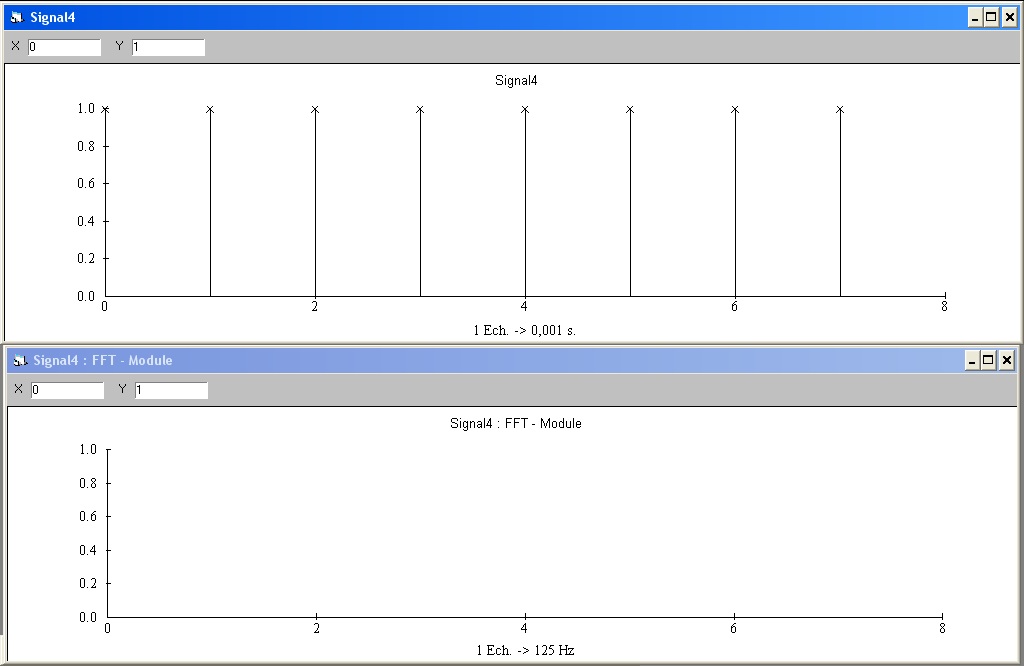
\includegraphics[width=10cm]{fig5.PNG}
		\caption{Signal Continu, 8 échantillons}
	\end{figure}
	L’impulsion de Dirac n’est pas visible puisqu’elle est confondue avec l’axe des ordonnées. Nous pouvons voir ce résultat avec les données X=0 et Y=1 en haut à gauche.\\
	
	Nous allons maintenant calculer la transformée de Fourier avec 16 échantillons.
	\begin{figure}[h]
		\centering
		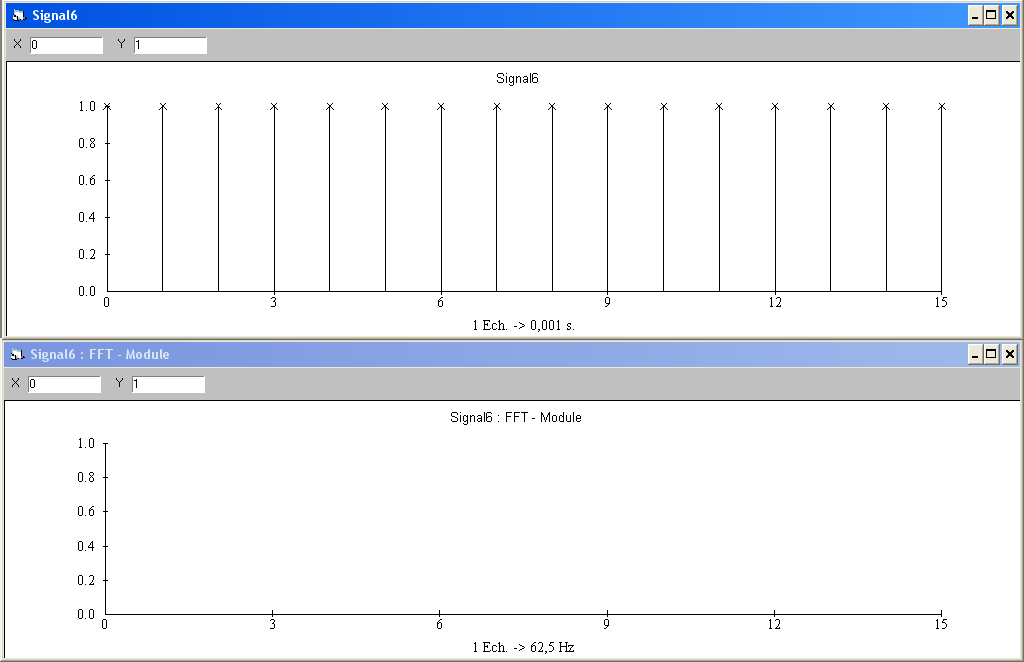
\includegraphics[width=10cm]{fig6.PNG}
		\caption{Signal Continu, 16 échantillons}
	\end{figure}
	Le résultat est le même que précédemment ce qui est le résultat attendu puisque la transformée ne dépend pas des paramètres d'échantillonnages du logiciel.\\
	\newpage
	\section{Signal rectangulaire symétrique}
	
	Nous allons maintenant travailler avec un signal rectangulaire symétrique d’amplitude +/- 1 V. L’objectif de cette partie est de regarder l’influence de la fréquence d’échantillonnage sur la qualité du spectre. Nous allons toujours travailler avec une seule période.\\

	\paragraph{Théorie}\paragraph{}
	Nous pouvons décomposer ce signal en la soustraction de deux portes. Une porte de largeur T d’amplitude 1 et une porte de largeur $\frac{T}{2}$ d’amplitude 2. Les portes n’étant pas centrées à l’origine, il faut donc prévoir un retard de $\frac{T}{4}$ pour avoir le même résultat que dans le logiciel.\\
	$$ f(t)=2rect(\frac{2t}{T})-rect(\frac{t}{T}) $$
	$$ TF(2rect(\frac{2t}{T})-rect(\frac{t}{T})) = T(sinc(\frac{\pi f T}{2}) - sinc(\pi f T)) $$
	$$ TF(2rect(\frac{2t}{T})-rect(\frac{t}{T})) = Te^{-\frac{j \pi f T}{2}}(sinc(\frac{\pi f t }{2}) - sinc(\pi f T) ) $$
	
	\paragraph{Pratique}\paragraph{}
	
	\begin{figure}[h]
		\centering
		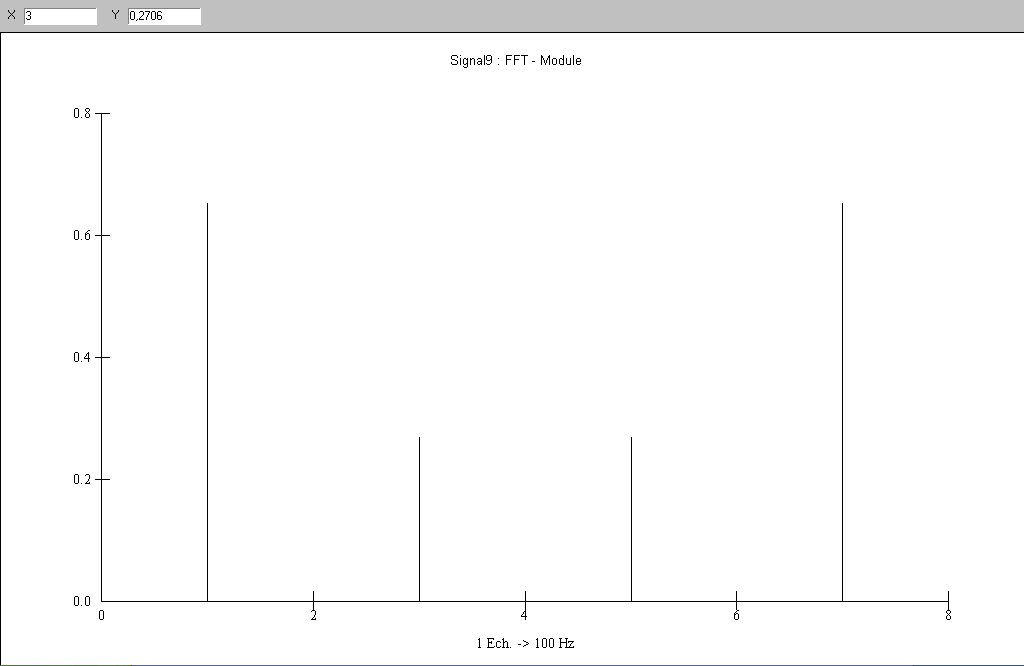
\includegraphics[width=10cm]{fig7.PNG}
		\caption{FFT d'un signal carré, 100Hz, 8 échantillons}
	\end{figure}
	\newpage

	\begin{figure}[h]
		\centering
		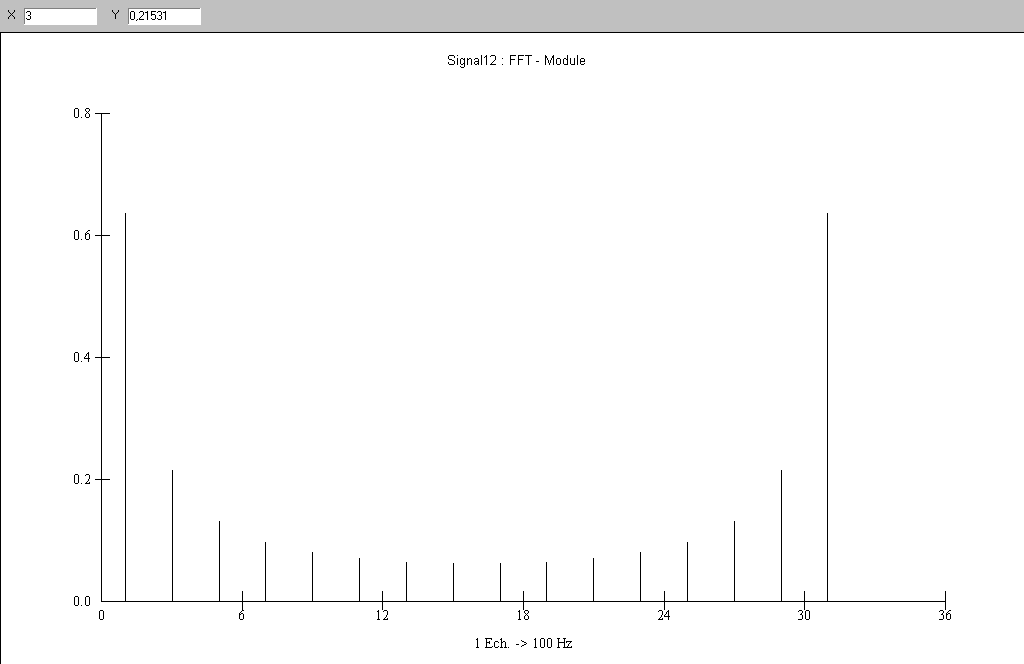
\includegraphics[width=10cm]{fig8.PNG}
		\caption{FFT d'un signal carré, 100Hz, 32 échantillons}
	\end{figure}

	\begin{figure}[h]
		\centering
		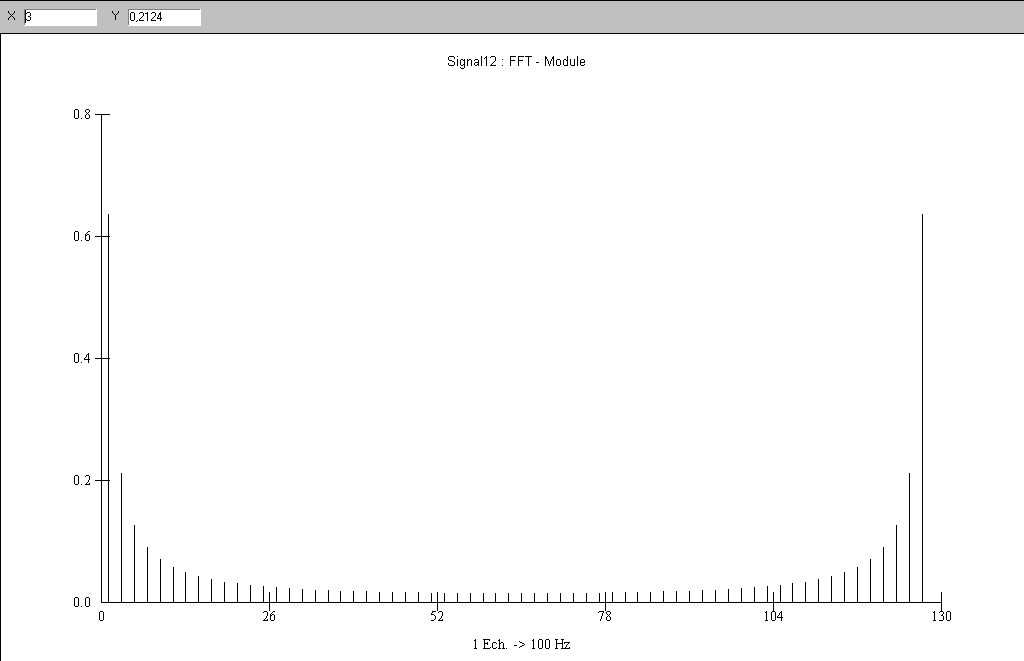
\includegraphics[width=10cm]{fig9.PNG}
		\caption{FFT d'un signal carré, 100Hz, 128 échantillons}
	\end{figure}
	\newpage
	
	Nous pouvons constater que sur les 3 figures précédentes que plus le nombre d’échantillons est important donc plus la fréquence d'échantillonnage est élevée plus la transformée obtenue est précise. Sur la première figure, il est impossible d'interpréter le résultat afin d’exploiter le signal. Sur la deuxième, nous commençons à distinguer la forme des exponentielles et sur le dernier nous la distinguons correctement.\\
	Ainsi, nous pouvons voir que si la fréquence d'échantillonnage n’est pas bien choisie, cela peut changer nos interprétation sur le signal. Le premier spectre pourrait être interprété comme le spectre d’un signal composé de deux sinus de fréquences différentes.
	\newpage
	\section{Créneau de durée déterminée}

	\paragraph{Théorie}\paragraph{}
	
	Un créneau de durée déterminée est semblable à une porte d’amplitude 1 et ayant une certaine ouverture.\\
	On a donc :
	$$ f(t) = rect(\frac{t}{T}) $$
	$$ TF(rect(\frac{t}{T})) = sinc(\pi f t)*T $$

	\paragraph{Pratique}\paragraph{}
	
	\begin{figure}[h]
		\centering
		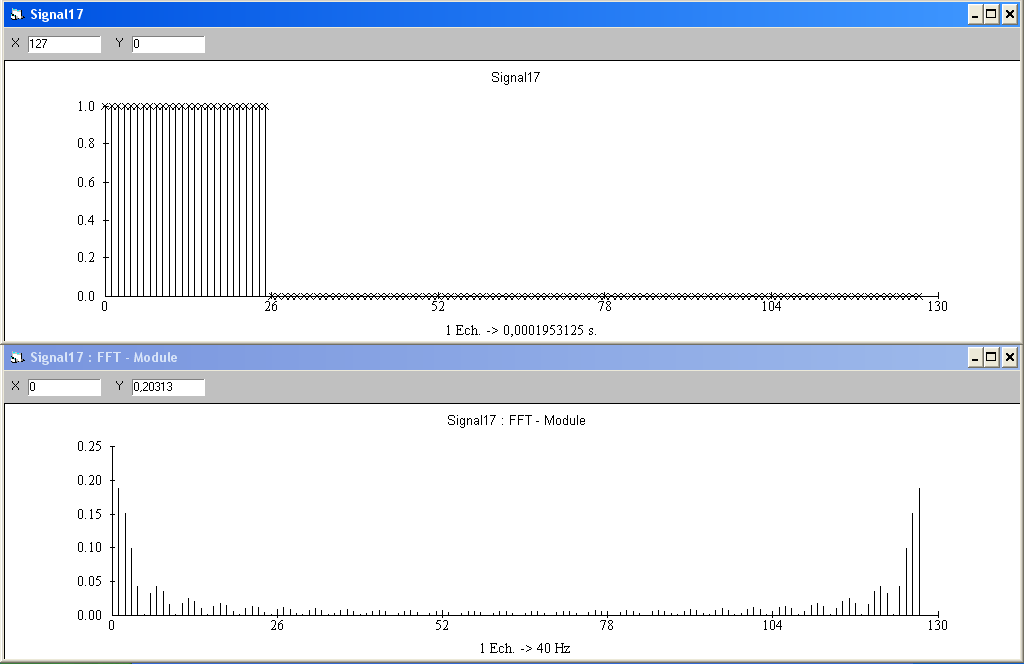
\includegraphics[width=10cm]{fig10.PNG}
		\caption{Porte simple à 128 échantillons}
	\end{figure}
	Afin de retrouver la forme du sinus cardinal, nous devons avoir une fréquence d'échantillonnage assez importante. Sachant que le nombre d’échantillons est de 128 et qu’ils sont tous espacés de 40 Hz, notre fréquence d’échantillonnage est donc de  5120 Hz.
	\newpage
	
	\begin{figure}[h]
		\centering
		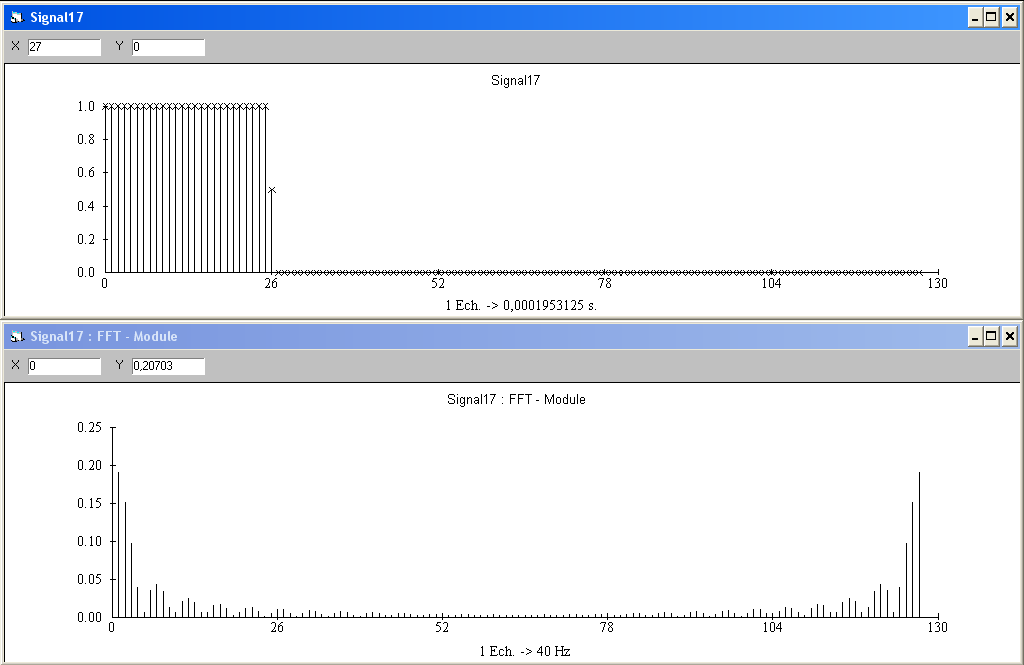
\includegraphics[width=10cm]{fig11.PNG}
		\caption{Porte avec transition à 128 échantillons}
	\end{figure}
	Ici nous voyons qu’en ajoutant une discontinuité, l’amplitude des raies de 50 à 80 est atténué.
	
	\begin{figure}[h]
		\centering
		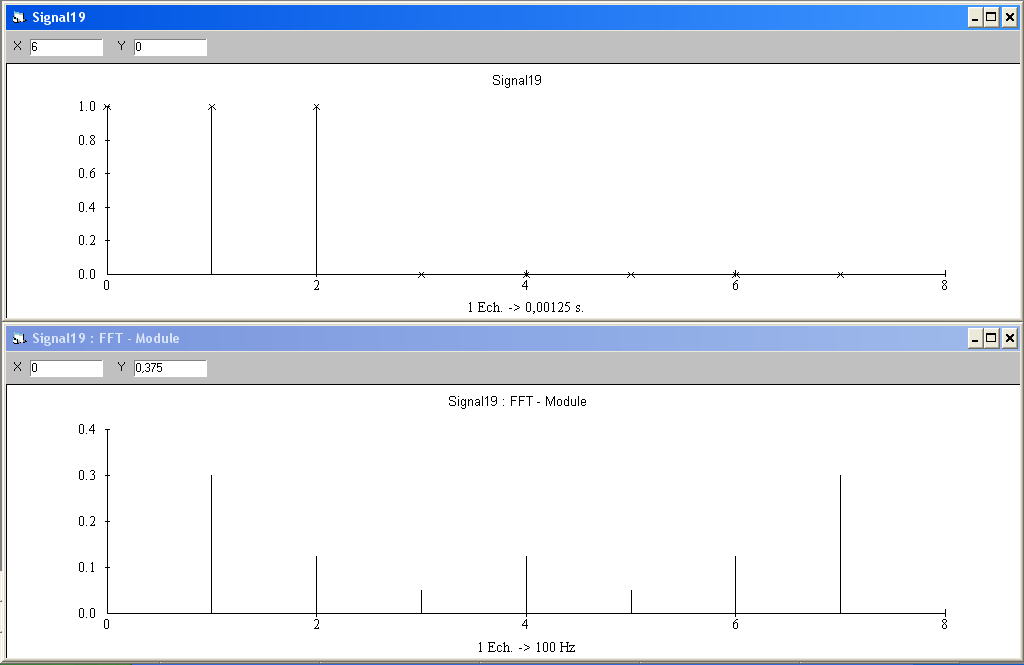
\includegraphics[width=10cm]{fig12.PNG}
		\caption{Porte simple à 8 échantillons}
	\end{figure}
	En passant le nombre d’échantillons à 8, le signal n’est plus reconnaissable. Nous voyons donc que le choix du nombre d’échantillons et donc de la fréquence d'échantillonnage est très important pour étudier correctement un signal.

\end{document}